\documentclass{beamer}
\usetheme{AnnArbor}
\usecolortheme{beaver}
\geometry{paperwidth=140mm,paperheight=105mm}
\usepackage[utf8]{inputenc}
\usepackage[T1]{fontenc}
\usepackage[italian]{babel}
\usepackage{soul}
\usepackage{graphicx}
\usepackage{algorithm2e}
\usepackage{multirow}

\usepackage{fancyvrb}
\definecolor{felinesrcbgcolor}{rgb}{1,1,0.85}
\definecolor{felinesrcbgcolor}{rgb}{0.94,0.97,1}
\definecolor{felineframe}{rgb}{0.79,0.88,1}
\definecolor{myorange}{rgb}{1,0.375,0}
\fvset{frame=lines,
  framesep=3mm,
  framerule=3pt,
  fontsize=\small,
  rulecolor=\color{myorange},
  formatcom=\color{DarkGreen},
}

\hypersetup{
	urlcolor=myorange
}

\title[Arch2013] % (optional, only for long titles)
{Architettura degli elaboratori 2012/2013}
\subtitle{Aritmetica binaria: Divisione Float e Float vs. C/C++}
\author{Michele ``Jazzinghen'' Bianchi\inst{1}}
\institute[DISI] % (optional)
{
  \inst{1}%
  Dipartimento di Ingegneria e Scienze dell'Informazione\\
  Universtià degli Studi di Trento
}
\date[2013-03-20] % (optional)
{20 Marzo 2013}
\subject{Computer Science, Embedded Systems}

\begin{document}
	\frame{\titlepage}
	\section{It's answer TIME!}
	\begin{frame}
    \frametitle{Alcune cose prima d'iniziare}
		\begin{itemize}
			\item La sottrazione può venir fatta sommando il complemento a
				2 solo se il numero di bit è limitato.
		  \item Quando facciamo operazioni con i float aggiungiamo zeri
		  		in fondo in modo da riempire tutti gli spazi della mantissa
		\end{itemize}
	\end{frame}   
  
	\section{Riassunto dell'ultima puntata}  
  \begin{frame}
    \frametitle{Cos'è successo l'ultima volta?}
		Abbiamo visto:    
    \begin{itemize}
    		\item Arrotondamento
    		\item Moltiplicazione
    		\item Somma
    		\item Sottrazione
    \end{itemize}
    %Unari, Babilonesi, Romani, Posizioniali (indiani), Binaria
  \end{frame}
	
	\section{Float Operations}
	\subsection{Divisione}
  \begin{frame}
    \frametitle{Floating Point}
    \framesubtitle{Divisione}       
    
    $$\frac{(-1)^{s1} \text{ } M1 \text{ } 2^{Exp1}}{(-1)^{s2} \text{ } M2 \text{ } 2^{Exp2}}= (-1)^{s} \text{ } M \text{ } 2^{Exp}$$
  	
  		\begin{center}
  			\begin{tabular}{|cc|}
  			\hline 
  			Segno (s) & s1 $\oplus$ s2 \\ 
  			\hline 
  			Valore (M) & $\frac{\text{M1}}{\text{M2}}$ \\ 
  			\hline 
  			Esponente (Exp) & Exp1 $-$ Exp2 \\ 
  			\hline 
  			\end{tabular} 
  		\end{center}
	  
	  \vspace{1em}
	  
	  Normalizzazione:
	  \begin{itemize}
	  		\item Se il numero è $> 1_{2}$ o $\geq 2_{10}$, shiftate a destra ed incrementate Exp di uno.
	  		\item Se l'esponente va oltre il massimo andiamo in \emph{overflow}
	  		\item Arrotondiamo il numero in modo che sia contenuto nella mantissa
	  \end{itemize}
  \end{frame}	  
  
  \begin{frame}
    \frametitle{Floating Point}
    \framesubtitle{Divisione tra interi}
    La parte peggiore della divisione tra float è dividere le due mantisse.
		
		\vspace{1em}
		    
    Vediamo prima come funziona la divisione tra interi:

		\vspace{1em}
		
		È uguale alla \emph{Divisione lunga} insegnata nelle scuole, la nostra
		fortuna, però, è che possiamo scegliere solo tra 1 e 0, quidi il divisore
		è o non è contenuto nelle cifre del dividendo che consideriamo ad ogni passaggio.
  \end{frame}
  
  	\subsection{Esempio di divisione base 10}
  \begin{frame}
	    \frametitle{Floating Point}
	    \framesubtitle{Esempio di divisione base 10}
				    
	    Iniziamo col fare una divisione banale in base 10.
	    
	    $$33_{10} / 6_{10} = ?$$
	    
	    \pause
	    \vspace{2em}
	    \begin{center}
	    		\setlength{\tabcolsep}{2pt}
	    		\begin{tabular}{cccccccc}
	    			3 & 3 & : & 6 & = & 5. & 5 \\
	    			3 & 0 &   &   &   &    &   \\
	    			\hline
	    			  & 3 & 0 &   &   &    &   \\
	    			  & 3 & 0 &   &   &    &   \\
	    			\hline
	    			  &   & - &   &   &    &   \\
	    		\end{tabular}
	    \end{center}
	    \pause
	    \vspace{2em}
	    $$33_{10} / 6_{10} = 5.5_{10}$$
	\end{frame}

	\subsection{Esempio di divisione base 2}
  \begin{frame}
	    \frametitle{Floating Point}
	    \framesubtitle{Esempio di divisione base 2}
				    
	    La divisione in base 2 funziona nella stessa maniera.
	    
	    $$100001_{2} / 110_{2} = ?$$
	    
	    \pause
	    \vspace{2em}
	    \begin{center}
	    		\setlength{\tabcolsep}{2pt}
	    		\begin{tabular}{ccc|cccccccc}
	    				&   &   &   &   &   & 1 & 0 & 1. & 1	\\
	    		  \hline    			
	    			1 & 1 & 0 & 1 & 0 & 0 & 0 & 0 & 1. & 0 \\
	    			  &   &   &   & 1 & 1 & 0 &   &   &    \\
	    			\hline
	    			  &   &   &   &   & 1 & 0 & 0 & 1 &    \\
	    			  &   &   &   &   &   & 1 & 1 & 0 &    \\
	    			\hline
	    			  &   &   &   &   &   &   & 1 & 1 & 0  \\
	    			  &   &   &   &   &   &   & 1 & 1 & 0  \\
	    			\hline
	    			  &   &   &   &   &   &   &   &   & -  \\
	    		\end{tabular}
	    \end{center}
	    \pause
	    \vspace{2em}
	    $$100001_{2} / 110_{2} = 101.1_{2}$$
	\end{frame}


	\subsection{Esempio di divisione float}
  \begin{frame}
    \frametitle{Floating Point}
    \framesubtitle{Esempio di divisione float}
    
		$$330_{10} / -0.625_{10} = ?$$
		
		\pause
		
		$330_{10} = 01000011101001010000000000000000$
		
		$-0.625_{10} = 10111111001000000000000000000000$
		
		\begin{center}
    		\setlength{\tabcolsep}{2pt}
    		\begin{tabular}{ccc|cccccccc}
    				&   &   & 1.& 0 & 0 & 0 & 0 & 1 & 0 & 0 \\
    		  \hline    			
    			1.& 0 & 1 & 1.& 0 & 1 & 0 & 0 & 1 & 0 & 1 \\
    			  &   &   & 1 & 0 & 1 &   &   &   &   &   \\
    			\hline
    			  &   &   &   &   & 0 & 0 & 0 & 1 & 0 & 1 \\
    			  &   &   &   &   &   &   &   & 1 & 0 & 1 \\
    			\hline
    			  &   &   &   &   &   &   &   &   &   & - \\
    		\end{tabular}
	  \end{center}		
		
		$$\text{M} = 00001000000000000000000$$ 
    
  \end{frame} 
  
  \begin{frame}
  	  \frametitle{Floating Point}
    \framesubtitle{Esempio di divisione float, cont.}
  	
    $$\text{Sign} = 0 \oplus 1 = 1$$
    
    $$\text{Exp} = 135 - 126 + 127 = 136_{10} = 10001000_{2}$$
    
    \pause
    \vspace{2em}
    
    $$11000100000001000000000000000000 = -528_{10}$$
  		
  \end{frame}
  \section{I Float e C/C++}
  \subsection{Le basi}
  \begin{frame}
  	  \frametitle{Floats vs. C/C++}
    \framesubtitle{I float nel C/C++}
  	
    Presenti due versioni del floating point:
    \begin{itemize}
    		\item \texttt{float}, 32-bit
    		\item \texttt{double}, 64-bit
    \end{itemize}
        
    \vspace{1em}
  		
  \end{frame}
  \subsubsection{Esponente e segno}
  \begin{frame}
  \frametitle{Esponente e segno}
  \framesubtitle{È stata dura, eh?}
  		
  		Esponente:
  		\vspace{1em}
  		$$(a*b^{x}) * (c * b^{y}) = (a*c) * (b^{x} * b^{y}) = (a*c) * b^{x+y}$$
  		
  		$$5_{10} + 6_{10} = 11_{10}$$
    
    $$\text{Exp} = 11_{10} + 127_{10} = 138_{10} = 10001010_{2}$$
   	Segno:
   	\vspace{1em}
    $$s = 0 \oplus 0 = 0$$
    
    \pause
		Struttura finale del float:    
    
    \vspace{1em}
   
    $32.375_{10} * 76.15625_{10} = 01000101000110100001100011110000$
  \end{frame}
  \subsection{Altro esempio}
  \begin{frame}
  		\frametitle{Altro esempio}
  		\framesubtitle{Partendo da due float}
  		Float 1: $10011011001001101011100000000000 = -1.379065_{10}*10^{-22}$
  		
  		Float 2: $01101000100010010010000000000000 = 5.1804360_{10}*10^{24}$
  		\vspace{2em}
  		\pause
  		\setlength{\tabcolsep}{2pt}
		\begin{center}
				\begin{tabular}{ccccccccccccccccccccccccc|c}
				  &   &   &   &   &   &   &   &   &   &   &   & 1.& 0 & 1 & 0 & 0 & 1 & 1 & 0 & 1 & 0 & 1 & 1 & 1 & x \\ 
				  &   &   &   &   &   &   &   &   &   &   &   & 1.& 0 & 0 & 0 & 1 & 0 & 0 & 1 & 0 & 0 & 1 &   &   & = \\ 
				\hline 
		      &   &   &   &   &   &   &   &   &   & 1 & 0 & 1 & 0 & 0 & 1 & 1 & 0 & 1 & 0 & 1 & 1 & 1 &   &   &   \\ 
          &   &   &   &   &   &   & 1 & 0 & 1 & 0 & 0 & 1 & 1 & 0 & 1 & 0 & 1 & 1 & 1 &   &   &   &   &   &   \\
  	        &   &   &   & 1 & 0 & 1 & 0 & 0 & 1 & 1 & 0 & 1 & 0 & 1 & 1 & 1 &   &   &   &   &   &   &   &   &   \\
  	      1 & 0 & 1 & 0 & 0 & 1 & 1 & 0 & 1 & 0 & 1 & 1 & 1 &   &   &   &   &   &   &   &   &   &   &   &   &   \\   
				\hline 
				  &   &   &   &   &   &   & 1 & 0 & 1 & 1 & 1 & 0 & 1 & 1 & 1 & 0 & 0 & 0 & 1 & 1 & 1 & 1 &   &   &   \\ 
				1 & 0 & 1 & 1 & 0 & 0 & 0 & 1 & 0 & 0 & 1 & 0 & 0 & 0 & 1 & 1 & 1 &   &   &   &   &   &   &   &   &   \\ 
				\hline 
				1.& 0 & 1 & 1 & 0 & 0 & 1 & 0 & 1 & 0 & 0 & 1 & 1 & 0 & 1 & 0 & 1 & 0 & 0 & 1 & 1 & 1 & 1 &  &    &   \\ 
				\end{tabular} 
		\end{center}
  \end{frame}
  \subsection{Limiti}
	\begin{frame}
    \frametitle{L'altro esempio}
    \framesubtitle{Segno, Esponente e poi mettere tutto assieme}
   		Exp 1: $00110110_{2} = 54$
   		Exp 2: $11010001_{2} = 209$
   		
   		$\text{Exp} = (\text{Exp 1} - \text{Bias}) + (\text{exp 2} - \text{Bias}) + \text{Bias} = (\text{Exp 1} + \text{Exp 2}) - \text{Bias}$
   		
   		$\text{Exp} = 54 + 209 - 127 = 136 = 10001000_{2}$
   		
   		\vspace{2em}
   		\pause
   		
   		Sign: $\text{Sign 1} \oplus \text{Sign 2} = 1 \oplus 0 = 1$
   		
   		\vspace{2em}
   		\pause
   		
   		Risultato:
   		\begin{columns}
				\column{.7\textwidth}   			
   			$$11000100001100101001101010011110 \simeq -714.4158_{10}$$
   			\column{.3\textwidth}
   			\pause
   			\begin{center}
		    		
\includegraphics[width=.9\textwidth]{IMGs/Everything.jpg}
		    \end{center}
			\end{columns}  
  \end{frame}
  \begin{frame}
  		\begin{center}
		  
\includegraphics[width=.6\textwidth]{IMGs/CoffeeTime.png}
		\end{center}
  \end{frame}
  \section{Intervallo}
	  \begin{frame}
	    \frametitle{Danni? Danni.}
	    \framesubtitle{Due errori piccoli non si annullano: ne fanno uno grosso.}
	    25 febbraio 1991. Prima guerra del Golfo, codename \emph{Operation: Desert Storm}.
	    
			\vspace{2em}	    
	    
	    A Dharan, in Arabia Saudita, c'è un accampamento americano protetto da una batteria \texttt{MIM-104} di
	    missili Patriot, progettati specificatamente come missili Terra-Aria con funzione
	    anti balistica.
	    
	    Quindi nessun problema, giusto?
	    
	    \pause
	    
	    \begin{center}
		    		
\includegraphics[width=.2\textwidth]{IMGs/no.jpg}
		    \end{center}
	    
	  \end{frame}
	  
	  \begin{frame}
	  		\frametitle{LOL, arrotondare}
	  	    
	    Quel giorno uno Scud iraqeno se ne passa indisturbato oltre l'area di rilevamento del sistema
	    e fa saltare in aria una caserma con 28 soldati e ne ferisce un centinaio.
	    
	    \vspace{2em}
	    \pause
	    
	    Nuove tecnologie segrete degli stati cagnaglia?
	    
	    \pause
	    
	    Delle spie che avevano disabilitato i sistemi di sicurezza?
	    
	    \pause
	    
	    Botta di sfiga?
	    
	    \pause
	    
	    \vspace{2em}
	    
	    No, ovviamente!
	    
	    Anche quì ci finiamo di mezzo noi.
	    
	  \end{frame}
	  
	  \begin{frame}
	  		\frametitle{LOL, arrotondare}
	    \framesubtitle{Vi ricordate la parte sui Fixed Points?}
	  	    
	    Fondamentalmente il sistema automatico di controllo dei \texttt{MIM-104}, per tenere traccia
	    del tempo, moltiplicava per 1/10 il tempo tracciato dall'orologio in tempo (che era in decimi).
	    
	    Per fare questo venivano utilizzati dei decimali in fixed points da 24 bits. Solo che, come ricorderete,
	    le operazioni con frazioni che non sono somme di potenze di due vengono "arrotondate" per specifiche. Un
	    bel modo per dire che non possiamo rappresentare questi numeri.
	    
	    $$0.10_{10} = 0.0001100110011001100110011001100\text{...}_{2}$$
	    
	    Noi, però, possiamo avvalerci solo di un numero finito di bit, quindi la rappresentazione a 24 bit sarà:
	    
	    $$0.00011001100110011001100_{2}$$
	    
	    Introducendo un errore, per ogni operazione, pari a:
	    
	    $$0.0000000000000000000000011001100\text{...}_{2} \simeq 0.000000095_{10}$$
	  \end{frame}
	  
	  \begin{frame}
	  		\frametitle{LOL, arrotondare}
	    \framesubtitle{L'uptime mi uccide.}
	  		
	  		
	    \begin{columns}
				\column{.6\textwidth}	
		  		Il sistema di controllo del \texttt{MIM-104} era acceso da oltre 100 ore.
		  		
		  		\vspace{2em}
		  		
		  		Ora, se fate due conti, questo vuol dire che l'errore accumulato era di
		  		
		  		$$100\text{h} * 60\frac{\text{m}}{\text{h}} * 60\frac{\text{s}}{\text{m}} * 10 * 0.000000095 = 0.342\text{s}$$
	    	    
	    	    \pause
		    Nice. In .342s uno Scud si fa circa 700m. Questo basta per fare in modo che un
				sistema non si accorga neanche della presenza del missile e non lo intercetti.
				
				youhadonejob.jpg
				\column{.4\textwidth}
				  \begin{center}
			    		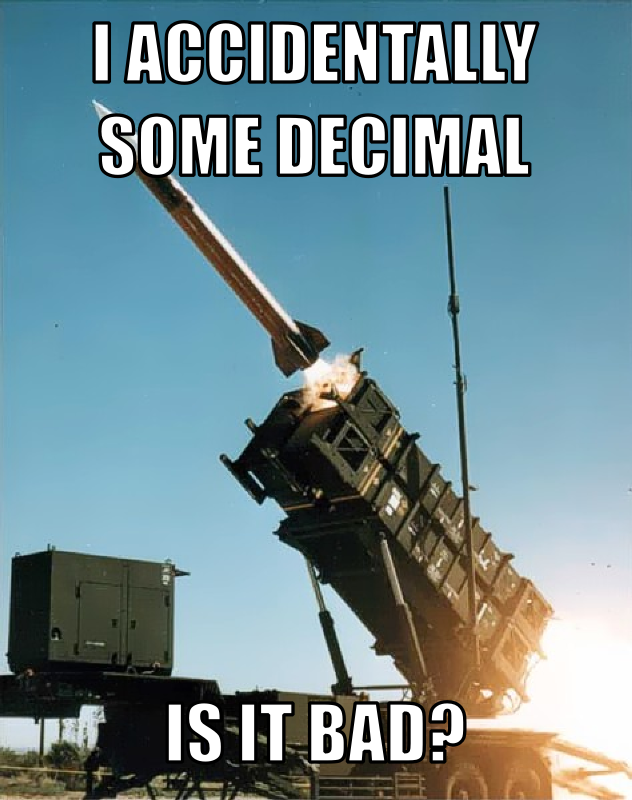
\includegraphics[width=.9\textwidth]{IMGs/Iaccidentally.png}
			    \end{center}
	    \end{columns}
	    
	  \end{frame}
	  
  \section{Float Operations - 2}
  \subsection{Somma/Sottrazione}
  \begin{frame}
    \frametitle{Floating Point}
    \framesubtitle{Somma}
      Anche quì l'idea di base è abbastanza semplice:
      $$(-1)^{s1} \text{ } M1 \text{ } 2^{Exp1} +_{f} (-1)^{s2} \text{ } M2 \text{ } 2^{Exp2} = (-1)^{s} \text{ } M \text{ } 2^{Exp}$$
      Per semplicità, nei calcoli, assumiamo che $\text{Exp1} \geq \text{Exp2}$
      \vspace{2em}
      
      Avremo quindi:
      \begin{itemize}
      		\item Exp = Exp1
      		\item S ed M saranno il risultato della somma (o sottrazione) dei due termini allineati
      \end{itemize}
      
      \vspace{2em}
      M andrà comunque normalizzata:
      \begin{itemize}
      		\item Se M$>1$ allora dobbiamo shiftare a destra, aumentando Exp di 1
      		\item Se M$<1$ allora dobbiamo shiftare a sinistra, diminuendo Exp di 1
      		\item Settiamo overflow ed arrotondiamo se necessario.
      \end{itemize}
      
  \end{frame}
	\subsection{Esempio Somma}
  \begin{frame}
    \frametitle{Floating Point}
    \framesubtitle{Esempio di somma}
    Float 1: $01000011101110100100000000000000 = 372.5_{2}$
    
    Float 2: $01000010101111101100000000000000 = 95.375_{2}$
    
    \pause
    \vspace{2em}
    
    Exp = Max(Exp1, Exp2) = Exp1 = 8
    
    M2 = $1.011111011_{2} * 2^{6} = 0.01011111011_{2} * 2^{8}$
    \vspace{1em}
    
    \setlength{\tabcolsep}{2pt}
    \begin{center}
    		\begin{tabular}{cccccccccccc|c}
    		1. & 0 & 1 & 1 & 1 & 0 & 1 & 0 & 0 & 1 &   &   & + \\ 
    		0. & 0 & 1 & 0 & 1 & 1 & 1 & 1 & 1 & 0 & 1 & 1 & = \\ 
    		\hline 
    		1. & 1 & 1 & 0 & 1 & 0 & 0 & 1 & 1 & 1 & 1 & 1 &   \\ 
    		\end{tabular} 
    \end{center}
    
    \pause 
    \vspace{1em}
    Risultato:
    $$01000011111010011111000000000000 = 467.875_{10}$$
  \end{frame}
  \subsection{Esempio Sottrazione}
  \begin{frame}
  		\frametitle{Floating Point}
  		\framesubtitle{Esempio di sottrazione}
  		Float 1: $01000101000101101100100000000000 = 2.4125_{10} * 10^{3}$
  		
  		Float 2: $11000110110110011101101000000000 = -2.7885_{10} * 10^{4}$
  		
  		\vspace{2em}
  		\pause
  		
    Exp = Max(Exp1, Exp2) = Exp1 = 14
    
    M2 = $1.001011011001_{2} * 2^{11} = 0.001001011011001_{2} * 2^{14}$
    \vspace{1em}
    
    \setlength{\tabcolsep}{2pt}
    \begin{center}
    		\begin{tabular}{cccccccccccccccc|c}
    		0. & 0 & 0 & 1 & 0 & 0 & 1 & 0 & 1 & 1 & 0 & 1 & 1 & 0 & 0 & 1 & + \\ 
    		0. & 0 & 1 & 0 & 0 & 1 & 1 & 0 & 0 & 0 & 1 & 0 & 0 & 1 & 1 & 0 & = \\ 
    		\hline 
    		0. & 0 & 1 & 1 & 1 & 0 & 0 & 0 & 1 & 1 & 1 & 1 & 1 & 1 & 1 & 1 &  \\
    		\hline
    		1. & 1 & 0 & 0 & 0 & 1 & 1 & 1 & 0 & 0 & 0 & 0 & 0 & 0 & 0 & 1 &  \\
    		\end{tabular} 
    \end{center}
    
    \pause 
    \vspace{1em}
    Risultato:
    $$11000110110001110000000100000000 = -2.54725_{10} * 10^{4}$$
  		
  \end{frame}
  \subsection{Divisione}
  \begin{frame}
  		\frametitle{Floating Point}
  		\framesubtitle{Divisione}
  		Lasciata per ultima perché io odio la divisione (E poi saltano in aria caserme).
  		
  		\vspace{2em}
  		\pause
  		
  		Voi non la odiavate alle ele... Med... Super... Vabbeh, quando si fa?
  		
  		\vspace{2em}
  		\pause
  		
  		È molto simile alla moltiplicazione, cambiano solo due cose:
  		\begin{itemize}
  			\item Fare la divisione invece che il prodotto tra le mantisse
  			\item Exp, alla fine, sarà (Exp1 - Exp 2) + Bias\footnote{Come mai?}
  		\end{itemize}
  		
  		Lo faremo la prossima volta.
  \end{frame}
% etc
\end{document}
